\documentclass[12pt]{../presentation}
%\documentclass[compress]{beamer}
\usetheme{default}
%\usecolortheme{whale}
\usepackage{ulem}
\usepackage{amsmath}
\usepackage{url}
\usepackage{graphicx}
\usepackage{pgf}
\usepackage{pgfplots}
\usepackage{tikz}
\usetikzlibrary{fit}					% fitting shapes to coordinates
\usetikzlibrary{backgrounds}	% drawing the background after the foreground
\usetikzlibrary{arrows,automata,calc,patterns,snakes}
\usepackage[latin1]{inputenc}
\usepackage{verbatim}
\usepackage{color, colortbl}

\newcommand{\vocab}{\mathbf{v}}
\newcommand{\dtvec}{\mathbf{t}_\Delta}
\newcommand{\ctxvec}{\mathbf{t}_\text{ctx}}
\newcommand{\dt}{\Delta_t}
\newcommand{\prerror}{Pr_{error}}
\newcommand{\fvec}{\mathbf{X}}
\newcommand{\weights}{\mathbf{w}}
\newcommand{\X}{\mathbf{X}}
\setbeamertemplate{footline}{\insertframenumber/\inserttotalframenumber}
\title{Predicting Web 2.0 Thread Updates}
\author{Shawn Tan}

\AtBeginSection[]
{
	\begin{frame}{Table of Contents}
	\tableofcontents[currentsection]
	\end{frame}
}
\date{}

\begin{document}
\maketitle
\section{Introduction}
\begin{frame}{Motivation}
	\begin{itemize}
		\item Many sites with thread-based discussion features
		\item Users post product reviews, feedback
	\end{itemize}
	Obtaining such up-to-date information may be vital to companies.
\end{frame}

\section{Related work}
\begin{frame}{Refresh policies for incremental crawlers}
Many works have used time difference to estimate page updates.
	\begin{enumerate}
		\item Coffman et. al. 1997 analysed the theoretical aspects.
		\item Cho and Garcia-Molina trace the change history of 720,000 web pages collected over 4 months.
		\begin{enumerate}		
			\item Showed empirically that the Poisson process model estimates the update processes well (Cho et. al. 1999)
			\item Proposed different revisiting or refresh policies (Cho et. al. 2003, Garcia-molina et. al. 2003)
		\end{enumerate}
		\item Also used in Tan et. al. 2007. %elaborate!!!!
	\end{enumerate}
\end{frame}

\begin{frame}{Problems with Poisson}
	The Poisson distribution is memoryless, and in experimental results due to Brewington and Cybenko 2000, the behaviour of site updates are not. 
\end{frame}

\begin{frame}{Using Site-level Knowledge}
Yang et. al. 2009, attempted to resolve this by
	\begin{enumerate}
		\item Using the list structure of forum sites to infer a sitemap.
		\item Use a linear-regression model to predict when the next update to the thread will arrive. %elaborate!!!
		\item Linear model used together with the sitemap information to prioritise the request queue in the crawler.
		\item Has the ability to make use of index information to infer changes in threads. Other types of comment systems do not have such indices.
	\end{enumerate}
\end{frame}

%TODO: New related work.
\begin{frame}{Summary}
	\begin{itemize}
		\item Previous work dealt with Web 1.0 sites.
		\item Did not take into account the content in the posts.
		\item Evidence to show that using time, while makes reasonable prediction, does not fully model the behaviour of threads.
	\end{itemize}
\end{frame}

\section{The Dataset}
\begin{frame}{avsforum.com}
	\begin{center}
		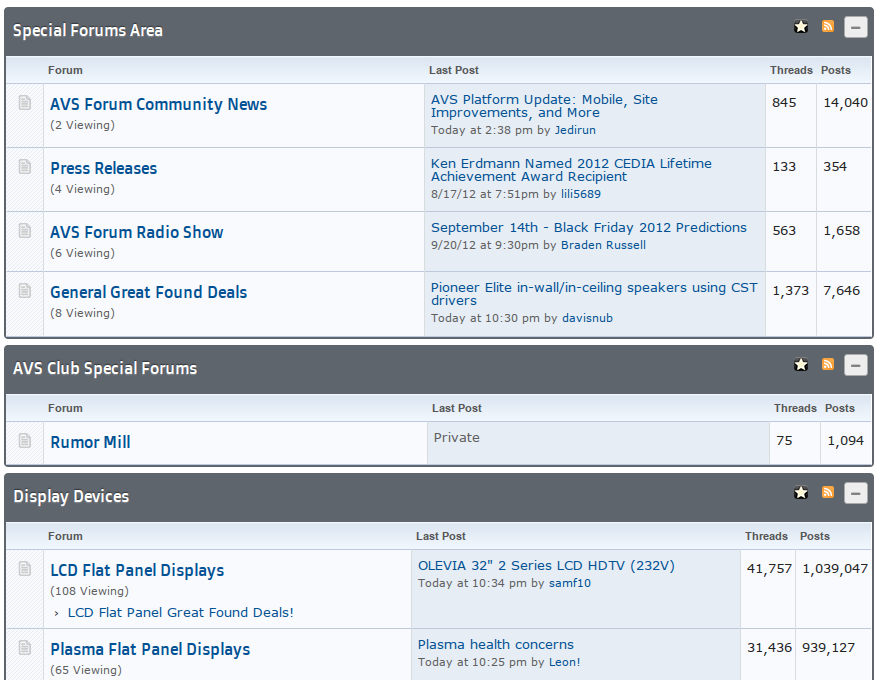
\includegraphics[scale=0.3]{screenshots/index.png}
	\end{center}
\end{frame}


\begin{frame}{User-centric threads}
	\begin{center}
		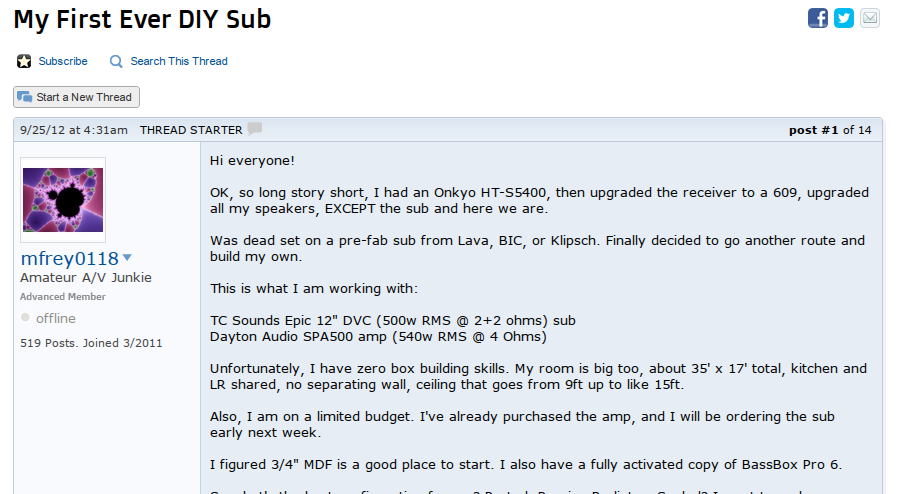
\includegraphics[scale=0.2]{screenshots/revolve_user.png}\\
			$\vdots$\\
		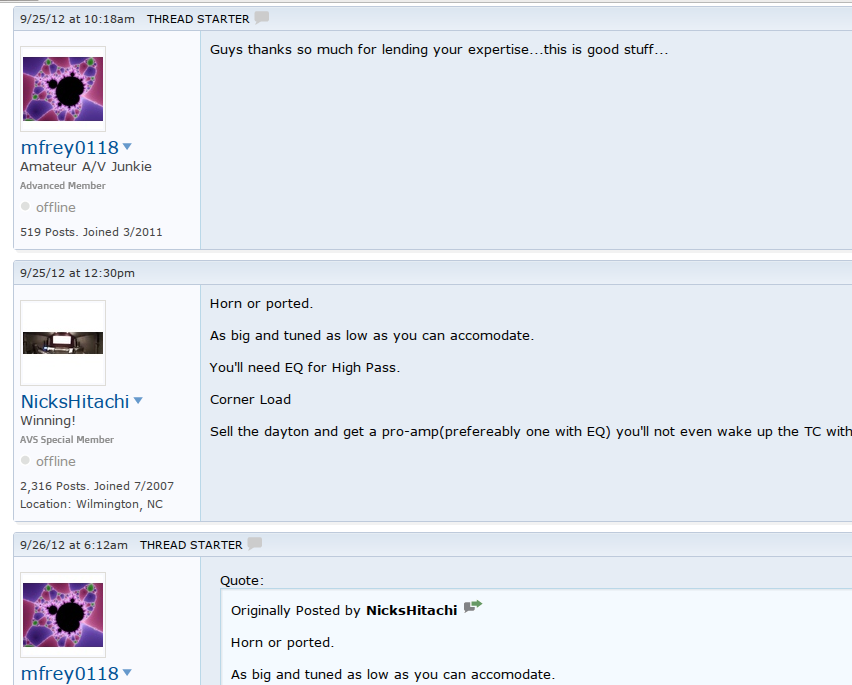
\includegraphics[scale=0.2]{screenshots/revolve_user2.png}
	\end{center}
\end{frame}


\begin{frame}{Questions}
	\begin{center}
		
\includegraphics[scale=0.4]{screenshots/question.png}\\
			$\vdots$\\
		
\includegraphics[scale=0.4]{screenshots/question2.png}
	\end{center}
\end{frame}
\begin{frame}{Mentions}
	\begin{center}
		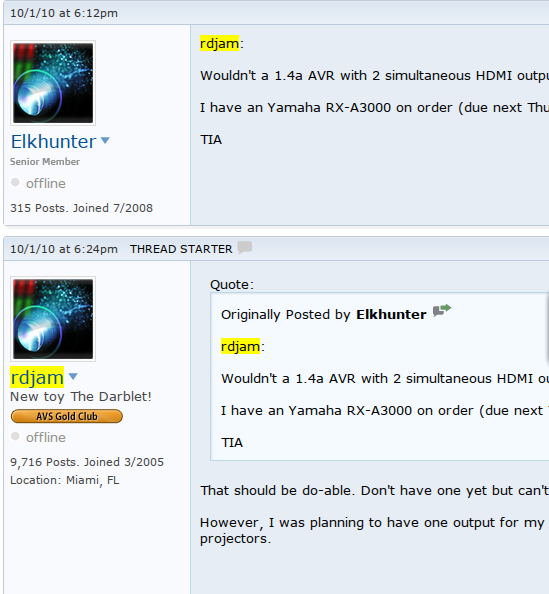
\includegraphics[scale=0.4]{screenshots/replies.png}\\
	\end{center}
\end{frame}


\section{Evaluation Metrics}
\begin{frame}{Requirements}
	\begin{itemize}
		\item Balance of freshness and bandwidth usage.
		\item Penalise when using too much bandwidth (visiting the site too 
			much).
		\item Penalise when ``database" not fresh (visiting the site too 
			little).
	\end{itemize}
\end{frame}

\begin{frame}{Events}
\begin{center}
	
\tikzstyle{background}=[rectangle,
	fill=gray!10,
	inner sep=0.2cm,
	rounded corners=5mm]


\tikzstyle{post}=[circle,
	thick,
	minimum size=1.2cm,
	draw=blue!80,
	fill=blue!20]
% The measurement vector is represented by an orange circle.
\tikzstyle{visit}=[circle,
	thick,
	minimum size=1.2cm,
	draw=orange!80,
	fill=orange!25]

\begin{tikzpicture}[>=latex,text height=1.5ex,text depth=0.25ex]
    % "text height" and "text depth" are required to vertically
    % align the labels with and without indices.
  
  % The various elements are conveniently placed using a matrix:
  \matrix[column sep=0.3cm] {
    % First line: Control input
    	&
		\node (e0)					{};&
		\node (e1)	[post]			{};&
		\node (e2)	[visit]			{};&
		\node (e3)	[post]			{};&
		\node (e4)	[visit]			{};&
		\node (e5)	[post]			{};&
		\node (e6)	[visit]			{};&
		\node (e)					{};&
		&
        \\
	};
    
    % The diagram elements are now connected through arrows:

	\path[-]
		(e0) edge[thick]	(e1)
		\foreach \e in {1,2,3,4,5}{
			let \n1={int(\e+1)} in (e\e) edge[thick] (e\n1)
		}
		(e6) edge[thick]	(e)
	;

	\begin{pgfonlayer}{background}
		\node [background,fit=(e1) (e3)] {};
	\end{pgfonlayer}

\end{tikzpicture}


\begin{tikzpicture}[>=latex,text height=1.5ex,text depth=0.25ex]
    % "text height" and "text depth" are required to vertically
    % align the labels with and without indices.
  
  % The various elements are conveniently placed using a matrix:
  \matrix[column sep=0.3cm] {
    % First line: Control input
    	&
		\node (e0)					{};&
		\node (e1)	[post]			{}; &
		\node (e2)	[visit]			{}; &
		\node (e3)	[post]			{}; &
		\node (e4)	[visit]			{}; &
		\node (e5)	[post]			{}; &
		\node (e6)	[visit]			{}; &
		\node (e)					{};&
		&
        \\
	};
    
    % The diagram elements are now connected through arrows:

	\path[-]
		(e0) edge[thick]	(e1)
		\foreach \e in {1,2,3,4,5}{
			let \n1={int(\e+1)} in (e\e) edge[thick] (e\n1)
		}
		(e6) edge[thick]	(e)
	;

	\begin{pgfonlayer}{background}
		\node [background,fit=(e3) (e5)] {};
	\end{pgfonlayer}

\end{tikzpicture}

\end{center}
\end{frame}
\begin{frame}{$T$-score}
\begin{center}
	\input{diagrams/t_score_diag}
\end{center}
\[
	T = \frac{1}{|P|} \sum^{|P|}_{i=1}\Delta t_i
\]
From Yang et. al. 2009
\end{frame}
\begin{frame}{Visit/Post ratio}
	\large
	Number of visits per post, keep the $T$-score in check.
\end{frame}

\begin{frame}{Normalised $T$-score}
	\begin{center}
		\input{diagrams/norm_t_score_diag}
	\end{center}
\end{frame}
\begin{frame}{Normalised Visit/Post ratio}
	\begin{center}
		\input{diagrams/fa_diag}
	\end{center}
\end{frame}

\section{Evaluation}
\begin{frame}{Experiment Setup}
{\scriptsize
\input{diagrams/exp_setup}}
For parameter tuning:
\begin{enumerate}
	\item Threads from 100 to 1000 posts
	\item 107 Threads in total
\end{enumerate}
\end{frame}

\begin{frame}{Baseline}
Take the average $\Delta_t$ from training set, and use that as the revisit time.
	\begin{center}
		\begin{tabular}{ | l | c | c | c | }
			\hline
		& $Pr_{error}$		  & $T$-score			   &	Visit/Post\\
			\hline
 Average &		0.501 $\pm$ 0.001 &	1764.474 $\pm$ 267.227  &	18.117 $\pm$ 7.290 \\
			\hline
		\end{tabular}
	\end{center}

\end{frame}

\begin{frame}{Windowing}
Use features from windows of posts. Number of posts in window given by $w$.
\begin{center}
\tikzstyle{background}=[rectangle,
	fill=gray!10,
	inner sep=0.2cm,
	rounded corners=5mm]


\tikzstyle{post}=[circle,
	thick,
	minimum size=0.75cm,
	draw=blue!80,
	fill=blue!20]
% The measurement vector is represented by an orange circle.
\tikzstyle{visit}=[circle,
	thick,
	minimum size=0.75cm,
	draw=orange!80,
	fill=orange!25]

\begin{tikzpicture}[>=latex,text height=1.5ex,text depth=0.25ex]
    % "text height" and "text depth" are required to vertically
    % align the labels with and without indices.
  
  % The various elements are conveniently placed using a matrix:
  \matrix[column sep=0.3cm] {
    % First line: Control input
    	&
		\node (e0)					{};&
		\node (e1)	[post]			{}; &
		\node (e2)	[visit]			{}; &
		&&
		\node (e3)	[post]			{}; &
		\node (e4)	[post]			{}; &
		&&
		\node (e5)	[visit]			{}; &
		\node (e6)	[post]			{}; &
		\node (e7)	[visit]			{}; &
		\node (e)					{};&
		&
        \\
	};
    
    % The diagram elements are now connected through arrows:

	\path[-]
		(e0) edge[thick]	(e1)
		\foreach \e in {1,2,3,4,5,6}{
			let \n1={int(\e+1)} in (e\e) edge[thick] (e\n1)
		}
		(e7) edge[thick]	(e)
	;
	\begin{pgfonlayer}{background}
		\only<1>{\node [background,fit=(e1) (e3)] {};}
		\only<2>{\node [background,fit=(e3) (e4)] {};}
		\only<3>{\node [background,fit=(e4) (e6)] {};}
    \end{pgfonlayer}


\end{tikzpicture}

\end{center}
\end{frame}


\begin{frame}{Window-based average}
	Take the average $\Delta_t$ from \sout{training set} the previous window, and use that as the revisit time.
	\begin{center}
		\scriptsize
		\begin{tabular}{ | l | c | c | c | c |}
			\hline
						&	        $T$-score &	       		Visit/Post	  & $Pr_{\text{error}}$\\
			\hline
		 $w = 5$		&	6420 $\pm$ 1000	&  16.6 $\pm$ 7 &	0.028 $\pm$ 0.005  \\
		 $w = 10$		&	4580 $\pm$ 700	&  17.4 $\pm$ 8 &	0.028 $\pm$ 0.005  \\
		 $w = 15$		&	3830 $\pm$ 600	&  18.5 $\pm$ 9 &	0.021 $\pm$ 0.003  \\
		 $w = 20$		&	3340 $\pm$ 400	&  18.3 $\pm$ 9 &	0.022 $\pm$ 0.004  \\
			\hline
		\end{tabular}
	\end{center}
	Performs worse than the simple average baseline.
\end{frame}

\begin{frame}{Support Vector Regression}
		Using only the window's $\Delta_t$ as features.
	\begin{center}
		\scriptsize
		\begin{tabular}{ | l | c | c | c | c |}
			\hline
						&	        $T$-score &	       		Visit/Post	  & $Pr_{\text{error}}$\\
			\hline
     $w=5 $ &	1537.682 $\pm$ 234.658	&  18.056 $\pm$ 7.585 &	0.018 $\pm$ 0.004  \\
     $w=10$ &	1485.157 $\pm$ 198.664	&  18.523 $\pm$ 8.028 &	0.019 $\pm$ 0.004  \\
     $w=15$ &	1433.771 $\pm$ 185.080	&  19.396 $\pm$ 8.896 &	0.016 $\pm$ 0.003  \\
     $w=20$ &	1577.639 $\pm$ 229.482	&  19.037 $\pm$ 8.690 &	0.019 $\pm$ 0.004  \\
			\hline
		\end{tabular}
	\end{center}
\end{frame}

\begin{frame}{Content-based features}
	Count of individual tokens used:
	\begin{enumerate}
		\item Text is stemmed, stopwords removed
		\item Occurences of usernames are replaced with `\#USER\#'
		\item Occurences of tokens with mixtures of alphabets and numbers are 
			replaced with `\#MODEL\#'
		\item Univariate regression tests used to select features
	\end{enumerate}
\end{frame}
\begin{frame}{Time-context}
	\begin{enumerate}
		\item Hour of the day
		\item Day of the week
	\end{enumerate}
	Represented as bit vectors
\end{frame}

\begin{frame}{Content features only}
	Using only the content features (stemmed word frequency counts).
	\begin{center}
		\footnotesize
	\begin{center}
		\scriptsize
		\begin{tabular}{ | l | c | c | c | c |}
			\hline
						&	        $T$-score &	       		Visit/Post	  & $Pr_{\text{error}}$\\
			\hline
 $w=5$	&	1593.380 $\pm$ 237.070	&  18.007 $\pm$ 7.585 &	0.019 $\pm$ 0.004  \\
$w=10$	&	1546.839 $\pm$ 198.243	&  18.493 $\pm$ 8.030 &	0.023 $\pm$ 0.006  \\
$w=15$	&	1491.695 $\pm$ 187.589	&  19.359 $\pm$ 8.899 &	0.021 $\pm$ 0.005  \\
$w=20$	&	1645.177 $\pm$ 232.365	&  19.017 $\pm$ 8.694 &	0.024 $\pm$ 0.005  \\
			\hline
		\end{tabular}
	\end{center}
	\end{center}
	Worse than the time difference approach, would using both sets of features help?
\end{frame}


\begin{frame}{Content features $+ \Delta_\mathbf{t} + $ time-context}
	\begin{center}
		\footnotesize
		\begin{tabular}{ | l | c | c | c | c |}
			\hline
						&	        $T$-score &	       		Visit/Post	  & $Pr_{\text{error}}$\\
			\hline
 $w=5$	&	1537.673 $\pm$ 234.657	&  18.056 $\pm$ 7.585 &	0.018 $\pm$ 0.004  \\
$w=10$	&	1485.137 $\pm$ 198.662	&  18.523 $\pm$ 8.028 &	0.019 $\pm$ 0.004  \\
$w=15$	&	1433.762 $\pm$ 185.078	&  19.396 $\pm$ 8.896 &	0.016 $\pm$ 0.003  \\
$w=20$	&	1577.639 $\pm$ 229.482	&  19.037 $\pm$ 8.690 &	0.019 $\pm$ 0.004  \\
			\hline
		\end{tabular}

	\end{center}
\end{frame}


\begin{frame}{Discounted Sum}
	Discounted sum of feature vectors from previous windows.
\[
	\X'_t = \X_t + \alpha \X'_{t-1}
\]
Where $0 \geq \gamma > 1$. Here we use only the word count as before.
	\begin{center}
		\footnotesize
		\begin{tabular}{ | l | c | c | c | }
			\hline
						&	        $T$-score &	       		Visit/Post	  & $Pr_{\text{error}}$\\
			\hline
		  $\alpha=1$ &	1433.761 $\pm$ 185.078 &   	19.396 $\pm$ 8.896 &  	0.002 $\pm$ 0.000 \\
          $\alpha=2$ &	1433.759 $\pm$ 185.078 &   	19.396 $\pm$ 8.896 &  	0.002 $\pm$ 0.000 \\
          $\alpha=3$ &	1433.757 $\pm$ 185.078 &   	19.396 $\pm$ 8.896 &  	0.002 $\pm$ 0.000 \\
          $\alpha=4$ &	1433.755 $\pm$ 185.077 &   	19.396 $\pm$ 8.896 &  	0.002 $\pm$ 0.000 \\
          $\alpha=5$ &	1433.755 $\pm$ 185.077 &   	19.396 $\pm$ 8.896 &  	0.002 $\pm$ 0.000 \\
          $\alpha=6$ &	1433.755 $\pm$ 185.077 &   	19.396 $\pm$ 8.896 &  	0.002 $\pm$ 0.000 \\
          $\alpha=7$ &	1433.755 $\pm$ 185.077 &   	19.396 $\pm$ 8.896 &  	0.002 $\pm$ 0.000 \\
          $\alpha=8$ &	1433.755 $\pm$ 185.077 &   	19.396 $\pm$ 8.896 &  	0.002 $\pm$ 0.000 \\
          $\alpha=9$ &	1433.746 $\pm$ 185.076 &   	19.396 $\pm$ 8.896 &  	0.002 $\pm$ 0.000 \\			
			\hline
		\end{tabular}
	\end{center}
\end{frame}
\begin{frame}{Stochastic Gradient Descent}
\begin{description}
	\item[Function to be fitted:]
\[
	f(\X) = \frac{\Lambda-\lambda}{1 + e^{\weights \cdot \X}} + \lambda
\]
\item[Update rule:]
\[
	\Delta \weights_i = \eta
				\underbrace{\left(\widehat{\dt} - \dt \right)}_{\text{error term}}
				\underbrace{\left( f(\X)(1-f(\X)) \right)}_{\text{gradient}}
						\X_i
\]
\end{description}
Update rule is used everytime a new post and time interval is observed.
\end{frame}

\begin{frame}{Scaled Sigmoid Function}
\begin{center}
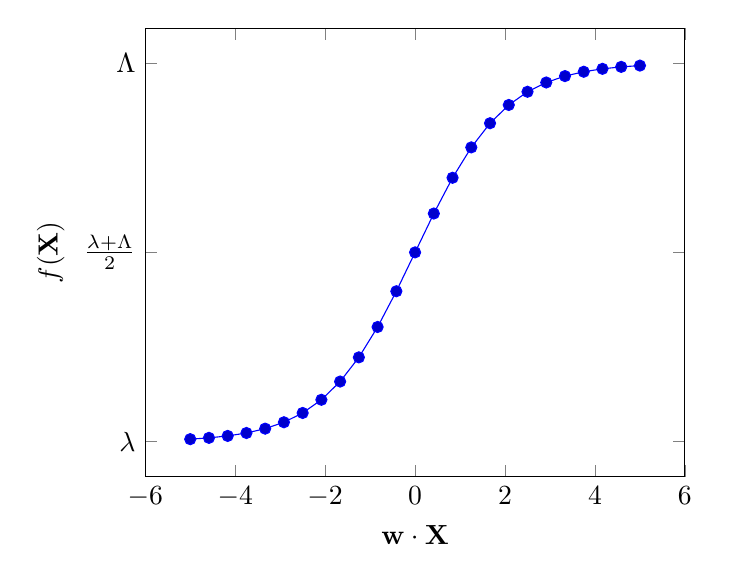
\begin{tikzpicture}
	\begin{axis}[
		xlabel=$\weights\cdot\X$,
		ylabel=$f(\X)$,
		ytick={0,0.5,1},
		yticklabels={$\lambda$,$\frac{\lambda + \Lambda}{2}$,$\Lambda$}
	]
\addplot {1/(1+ e^-x)}; \end{axis}
\end{tikzpicture}
\end{center}
\end{frame}

\begin{frame}{SGD results}
	\begin{center}
		\footnotesize
		\begin{tabular}{ | l | c | c | c | }
			\hline
				  & $T$-score			   &	Visit/Post\\
			\hline
	$\eta=5\cdot10^{-5}$ &	1595.563 &	    19.097 \\
	$\eta=5\cdot10^{-6}$ &	1525.705 &	    19.122 \\
	$\eta=5\cdot10^{-7}$ &	1440.440 &	    19.121 \\
\rowcolor{green}
	$\eta=5\cdot10^{-8}$ &	1407.172 &	    19.108 \\
	$\eta=5\cdot10^{-9}$ &	1416.182 &	    19.110 \\
	$\eta=5\cdot10^{-10}$ &	1451.729 &	    19.106 \\
	$\eta=5\cdot10^{-11}$ &	1482.868 &	    19.104 \\
	$\eta=5\cdot10^{-12}$ &	1487.555 &	    19.104 \\
			\hline
		\end{tabular}
	\end{center}
\end{frame}
\begin{frame}{Wilcoxon's signed-rank test}
Cannot use Student's $t$ test, since distribution of $T$-scores is not normal
\begin{itemize}
\item Non-parametric statistical hypothesis test
\item Data paired, and come from same population
\item $H_0:$ No difference between my model and baseline (average time revisitation)
\item $H_1:$ My model performs better than baseline
\end{itemize}	
\end{frame}

\begin{frame}{Results of Paired Tests}
	\begin{center}\begin{tabular}{l l}
		$T$-score 	 & -381.885 $\pm$ 153.673\\
		Visit/Post 	 & 1.053 $\pm$ 1.749	   \\
\rowcolor{green}
		Single-sided test & 0.0486 \\
	\end{tabular}\end{center}
\end{frame}

\begin{frame}{Analysis of Data}
What words are important, and how do they change over time?

How does the number of posts used to train the model affect the result?
\end{frame}


\begin{frame}{Limitations}
	\begin{enumerate}
		\item Experiments only performed on one forum
		\item (In)Correctness of model
		\item Stochastic Gradient Descent is slow
	\end{enumerate}
\end{frame}

\begin{frame}{Future Work}
	\begin{enumerate}
		\item Incorporate decay into model
			\begin{itemize}
				\item SVM with adaptive parameters (Cao \& Tay, 2003)
			\end{itemize} 
		\item NLP techniques
			\begin{itemize}
				\item Use features from Wang, Chen, and Kan (2012)
			\end{itemize} 
		\item Lexical Chaining
			\begin{itemize}
				\item Wang and McCarthy (2011)
			\end{itemize}
	\end{enumerate}
\end{frame}


\begin{frame}
	\begin{center}
		\large 
		Questions? Suggestions?
	\end{center}
\end{frame}

\end{document}
